\documentclass[a4paper, 14pt]{article}
\usepackage[margin=1.6cm]{geometry}
\usepackage[utf8]{inputenc}
\usepackage{minted}
\usepackage[russian]{babel}
\usepackage{amsmath}
\usepackage{graphicx}
\usepackage{changepage}
\usepackage{hyperref}
\usepackage{cases}
\pagestyle{empty}

\hypersetup{
	linkbordercolor = {1 1 1}
}

\usepackage[usenames,dvipsnames,svgnames,table]{xcolor}
\usepackage{tikz-timing}[2009/05/15]
\usepackage{multicol}
\usepackage[T2A]{fontenc}
\usepackage{pgfplots}
%\usepackage[left=2.5cm, right=1.5cm, vmargin=2.5cm]{geometry}
\setlength\parindent{0pt} % Удалить отступы из параграфов.

\usepackage{listings}
\usepackage{caption}
\DeclareCaptionFont{white}{\color{white}} % Текст заголовка.
\DeclareCaptionFormat{listing}{\colorbox{gray}{\parbox{\textwidth}{#1#2#3}}}
\captionsetup[lstlisting]{format=listing,labelfont=white,textfont=white}
\renewcommand\labelenumi{\theenumi)}



\begin{document}
\lstset{
	language=java,                 % Выбор языка для подсветки (здесь это java).
	basicstyle=\small\sffamily,    % Размер и начертание шрифта для подсветки кода.
	numbers=left,                  % Где поставить нумерацию строк (слева\справа).
	numberstyle=\tiny,             % Размер шрифта для номеров строк.
	stepnumber=1,                  % Размер шага между двумя номерами строк.
	firstnumber=1,
	numberfirstline=true
	numbersep=5pt,                 % Как далеко отстоят номера строк от подсвечиваемого кода.
	backgroundcolor=\color{white}, % Цвет фона подсветки - используем \usepackage{color}.
	showspaces=false,              % Показывать или нет пробелы специальными отступами.
	showstringspaces=false,        % Показывать или нет пробелы в строках.
	showtabs=false,                % Показывать или нет табуляцию в строках.
	frame=single,                  % Рисовать рамку вокруг кода.
	tabsize=2,                     % Размер табуляции по умолчанию равен 2 пробелам.
	captionpos=t,                  % Позиция заголовка вверху [t] или внизу [b].
	breaklines=true,               % Автоматически переносить строки (да\нет).
	breakatwhitespace=false,       % Переносить строки только если есть пробел.
	escapeinside={\%*}{*)}         % Если нужно добавить комментарии в коде.
}

\begin{titlepage}
	\center

	ФЕДЕРАЛЬНОЕ ГОСУДАРСТВЕННОЕ АВТОНОМНОЕ ОБРАЗОВАТЕЛЬНОЕ УЧРЕЖДЕНИЕ ВЫСШЕГО ОБРАЗОВАНИЯ\linebreak
	«Санкт-Петербургский политехнический университет Петра Великого»\\[1cm]
	\textsc{\Large Институт компьютерных наук и технологий}\\
    \textsc{\large Высшая школа программной инженерии}\\[3.5cm]

	{ \huge \bfseries КУРСОВАЯ РАБОТА	\\
	\Large \mdseries ОПРЕДЕЛЕНИЕ РАССТОЯНИЯ ДО ОБЪЕКТА ПУТЕМ УЛЬТРАЗВУКОВОГО ИЗМЕРЕНИЯ С ПОМОЩЬЮ HC-SR04 \\
	\large по дисциплине <<Микропроцессорные системы>>}\\[6.5cm]


	\begin{multicols}{2}
		\begin{flushright} \large

			{Выполнили студенты группы: 3530904/00104:}\\
            {\phantom{qwe}}\\
            {\phantom{qwe}}\\
            {\phantom{qwe}}\\
            {\phantom{qwe}}\\

			{Преподаватель:\\}

		\end{flushright}
		\begin{flushright}

			{Пятизбянцев И. А.}\\
			{Мурзаканов И. М.}\\
			{Поздняков А. А.}\\
			{Почернин В. С.}\\
			{Шиляев В. С.}\\[0.5cm]


			Круглов С. К.\\

		\end{flushright}
	\end{multicols}

	\flushright{
        {\phantom{qwe}}\\[4.5cm]
		{\today}\\
	}
	\centering{
		Санкт-Петербург\\
		2022
	}

	\vfill
\end{titlepage}

\large
\tableofcontents
\newpage

\section{Условие задачи}

Поставленная задача: разработать и собрать систему на базе платы с процессором ARM, которая позволит измерить расстояние до объекта с помощью ультразвукового датчика.

\newpage
\section{Используемое оборудование}

При выборе основной платы была выбрана Raspberry Pi. В нашем случае в качестве операционной системы используется Raspbian OS - родной дистрибутив для платы. Таким образом на данной плате мы можем не только запустить проект, но и вывести результаты благодаря подключению по SSH.

Ниже представлены технические характеристики:

\begin{itemize}
    \item Процессор: Quad core Cortex-A72 (ARM v8) 64-bit SoC @ 1.5GHz;
    \item Оперативная память: 4GB LPDDR4-2400 SDRAM;
    \item Цифровой видеовыход: HDMI;
    \item Композитный выход: 3.5 мм (4 pin);
    \item USB порты: USB 2.0 x4;
    \item Сеть: WiFi 802.11n, 10/100 Мб RJ45 Ethernet;
    \item Bluetooth: Bluetooth 4.1, Bluetooth Low Energy;
    \item Разъем дисплея: Display Serial Interface (DSI);
    \item Карта памяти: MicroSD;
    \item Порты ввода-вывода: 40;
    \item HC-SR04 Ultrasonic Range Sensor;
    \item $1k\Sigma$ резистор;
    \item $2k\Sigma$ резистор;
    \item Провода джамперы;
\end{itemize}

\newpage
\section{Ультразвуковые датчики расстояния}

\begin{figure}[H]
	\centering
	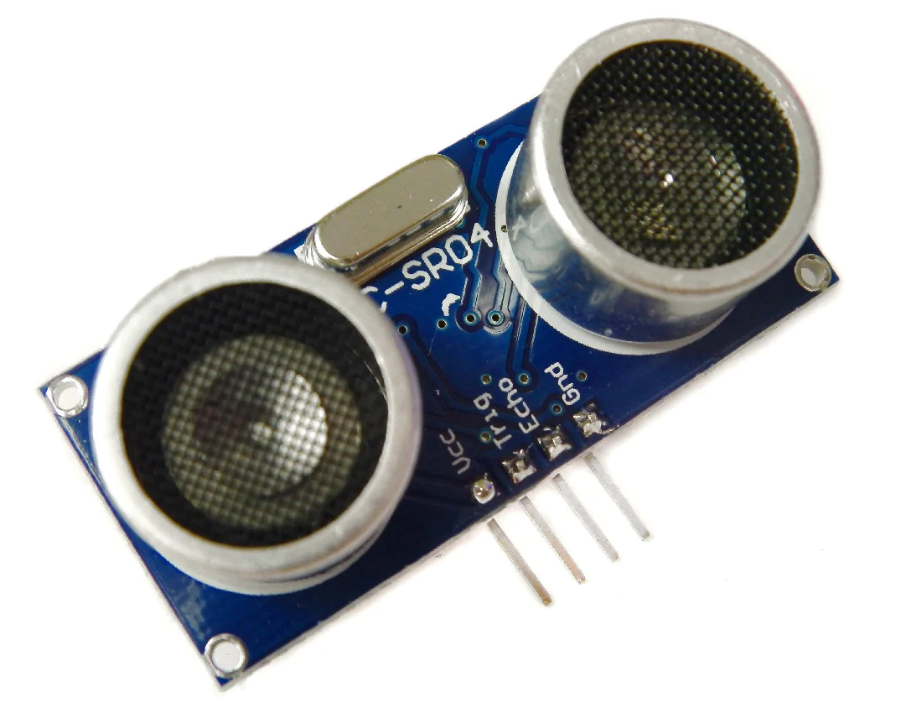
\includegraphics[width=15cm]{screenshots/1.png}\\
	\caption{Ультразвуковой датчик HC-SR04}
\end{figure}

Звук состоит из колеблющихся волн в среде (например, в воздухе), высота звука которых определяется близостью этих волн друг к другу, определяемой, как \textbf{частота}.

\newpage
\section{Схема устройства}

\newpage
\section{Raspberry Pi 4B. Удаленное управление через SSH}

\newpage
\section{Результаты работы}

\newpage
\section{Выводы}

\newpage
\section{Исходные тексты программ}

\newpage
\section{Список литературы и электронных источников}

\end{document}